\documentclass[11pt]{article}

\usepackage[utf8]{inputenc}
\usepackage[T1]{fontenc}
\usepackage[margin=1in]{geometry}
\usepackage{amsmath,amssymb,amsthm}
\usepackage{booktabs}
\usepackage{graphicx}
\usepackage{xcolor}
\usepackage{tikz}
\usetikzlibrary{arrows.meta,positioning,calc,shapes.geometric,fit,backgrounds}
\usepackage[font=small,labelfont=bf]{caption}
\usepackage{subcaption}
\usepackage{algorithm}
\usepackage{algpseudocode}
\usepackage{hyperref}
\usepackage{natbib}
\hypersetup{colorlinks=true,linkcolor=blue!50!black,citecolor=blue!50!black,urlcolor=blue!50!black}

\newcommand{\code}[1]{\texttt{#1}}

\title{Scaling Portfolio-Level Reinforcement Learning\\
       via Anchor-Token Cross-Attention}
\author{Prabal Negi \\ \small \texttt{market-agent} project \\[2pt]
        \small Architecture analysis and manuscript drafted with Claude (Anthropic)}
\date{September 2026}

\begin{document}
\maketitle

\begin{abstract}
\noindent
\texttt{TradingGame} is a rule-constrained portfolio-management reinforcement
learning environment: an actor-critic policy chooses buy/sell/hold actions
jointly across a candidate universe of $N$ stocks under a shared cash
constraint, trained with Proximal Policy Optimization (PPO). The current
policy network aggregates cross-candidate context with full self-attention
over all $N$ candidates plus a portfolio token, an $O(N^2)$ operation. This
note (i) formalizes the environment and the existing architecture, (ii)
reports a direct empirical characterization of that architecture's GPU memory
footprint --- thirteen measurements on real hardware, fitted to a closed-form
model with $R^2 = 0.9999999$ --- showing the design cannot reach a
$N{=}1{,}500$-company universe at useful batch sizes, and (iii) proposes an
$O(N(K{+}2))$ replacement, \emph{anchor-token cross-attention}, in which each
candidate attends only to a small fixed set of $K$ real anchor stocks plus
separate macro and portfolio tokens, rather than to every other candidate or
to a single pooled summary. We show the redesign is necessary but not
sufficient: removing the quadratic term exposes a previously-dominated linear
term, whose coefficient we also measure directly, giving a closed-form bound
on the batch size the redesign alone can reach at a given $N$.
\end{abstract}

\tableofcontents

% ─────────────────────────────────────────────────────────────────────────
\section{Introduction}

\texttt{TradingGame} trains a single reinforcement-learning policy to manage
a simulated portfolio of Indian (NSE/BSE) equities under an explicit rule
set: a fixed starting cash balance; a 0.5\% fee on every transaction; sale
proceeds that settle into spendable cash only after a two-trading-day delay;
a one-trading-day lock-up before a newly-bought lot can be voluntarily sold
again; and an unconditional forced exit after ten trading days. The policy
observes a capped \emph{candidate universe} of $N$ stocks at each decision
step and must choose, jointly, which to hold, sell, or buy --- subject to a
single shared cash pool, so the decisions are coupled across candidates, not
independent per-stock classifications.

The current implementation (\code{ActorCriticPolicy} in
\code{packages/TradingGame/src/policy.jl}) caps $N$ at 60. Growing the
candidate universe toward index scale ($N \approx 1{,}500$) is desirable for
realistic diversification, and is newly plausible now that training runs on
a dedicated GPU rather than CPU alone. Section~\ref{sec:baseline} shows why
the current architecture cannot simply be pointed at a larger $N$: its
cross-candidate attention mechanism is quadratic in $N$. Section~\ref{sec:measurement}
characterizes that cost directly, on real hardware, rather than by asymptotic
argument alone. Section~\ref{sec:proposed} derives a linear-cost
replacement, and Section~\ref{sec:linear-bottleneck} shows why that
replacement is a necessary but incomplete fix.

% ─────────────────────────────────────────────────────────────────────────
\section{Related Work}
\label{sec:related}

\paragraph{Self-attention and its cost.} Scaled dot-product self-attention
\citep{vaswani2017attention} lets every element of a set condition on every
other element, at $O(n^2)$ time and memory in the set size $n$. This is the
mechanism the current \texttt{ActorCriticPolicy} uses across candidates.

\paragraph{Reducing attention to sub-quadratic cost.} Several strategies
replace all-pairs attention with attention against a smaller, fixed
reference set. \citet{lee2019settransformer} introduce the \emph{Induced Set
Attention Block} (ISAB): rather than $n$ elements attending to all $n$
others, they attend to $m \ll n$ learned \emph{inducing points}, reducing
cost from $O(n^2)$ to $O(nm)$ while remaining a permutation-invariant
function of the input set --- exactly the structure we adopt in
Section~\ref{sec:proposed}, with the inducing points replaced by a
small set of \emph{real, interpretable} anchor stocks. Other lines of work
achieve sub-quadratic attention via low-rank projection of the sequence
dimension \citep{wang2020linformer} or kernel approximations of the softmax
\citep{choromanski2021performer}; we do not adopt these here because they
trade the interpretability of "which stocks is candidate $i$ attending to"
for a compressed or randomized basis, which is a poor fit for a financial
decision system where that interpretability is itself valuable.

\paragraph{Recurrent per-element encoders.} Each candidate's own price
history is encoded independently with a Gated Recurrent Unit
\citep{cho2014gru} before any cross-candidate mixing; this per-candidate
encoding is where the dominant \emph{linear}-in-$N$ cost identified in
Section~\ref{sec:linear-bottleneck} originates, and it is unaffected by
whichever cross-candidate attention pattern is used downstream.

\paragraph{Combined policy/value networks trained by self-play or
policy-gradient RL.} AlphaGo Zero and its generalization
\citep{silver2017agz,silver2018alphazero} share a trunk between a policy head
and a value head, trained end-to-end --- the same actor-critic head
structure \texttt{ActorCriticPolicy} uses, though those systems operate over
a fixed-size board rather than a variable, rule-constrained financial action
space. We train with Proximal Policy Optimization
\citep{schulman2017ppo} and Generalized Advantage Estimation
\citep{schulman2016gae}, in the tradition of actor-critic methods such as
A3C \citep{mnih2016a3c}; optimization uses Adam \citep{kingma2015adam}.
\citet{lecun2015deeplearning} give a general account of the representation
learning this architecture relies on throughout.

\paragraph{Internal precedent.} This repository's own
\texttt{StockSwingPredictor} package made the analogous choice once before,
for a different model: its first architecture (\code{DualCNN\_v1}) aggregated
a target stock's peer context by \emph{mean-pooling} up to 150 peer
embeddings; the second (\code{DualCNN\_v2}) replaced that pooling with
cross-attention, specifically because a flat average cannot express
\emph{which} peers matter for a given target. Section~\ref{sec:proposed}
applies the identical argument to \texttt{TradingGame}: an earlier draft of
this proposal itself made the mean-pool mistake it is meant to avoid, by
aggregating all $N$ candidates into one pooled "market pulse" token before
realizing this reintroduced exactly the selectivity loss that motivated
\code{DualCNN\_v2} in the first place.

% ─────────────────────────────────────────────────────────────────────────
\section{Environment and Decision Problem}
\label{sec:mdp}

We formalize the rules enforced by \code{packages/TradingGame/src/env.jl}
(\texttt{TradingGameRules.txt}, repo root) as a discrete-time Markov decision
process.

\paragraph{Portfolio state.} At trading-hour index $t$, the portfolio holds
spendable cash $C_t$, a set of reserved-cash lots
$\mathcal{R}_t = \{(\rho_k, \tau_k)\}$ (amount, maturity trading-day index),
and a set of open lots $\mathcal{L}_t = \{(i_\ell, q_\ell, p_\ell, d_\ell)\}$
(stock index, quantity, entry price, entry trading-day index). Portfolio
value is
\begin{equation}
  V_t \;=\; C_t \;+\; \sum_{(\rho,\tau)\in\mathcal{R}_t}\rho
       \;+\; \sum_{(i,q,p,d)\in\mathcal{L}_t} q \cdot P_{i,t},
  \label{eq:portfolio-value}
\end{equation}
where $P_{i,t}$ is stock $i$'s price at $t$ --- rules 2 and 6 of
\texttt{TradingGameRules.txt}, restated identically.

\paragraph{Settlement, lock-up, forced exit.} Let $\delta(t)$ be the trading-day
index of hour $t$. A reserved-cash lot $(\rho,\tau)$ matures --- moves into
$C_t$ --- once $\delta(t) \ge \tau$, with $\tau = \delta(t_{\text{sell}}) +
\tau_{\text{settle}}$, $\tau_{\text{settle}}=2$ (rule 4). A lot
$(i,q,p,d)$ may be voluntarily sold only once $\delta(t) - d \ge
\tau_{\text{lock}}$, $\tau_{\text{lock}}=1$ (rule 9), and is
\emph{unconditionally} liquidated once $\delta(t) - d \ge \tau_{\text{max}}$,
$\tau_{\text{max}}=10$ (rule 8), independent of the policy's action.

\paragraph{Action space.} At each decision step the policy emits, jointly
for every candidate $i \in \{1,\dots,N\}$, a discrete type and a continuous
weight:
\begin{equation}
  a_t \;=\; \big(a^{\text{type}}_{i,t},\, w_{i,t}\big)_{i=1}^{N},
  \qquad a^{\text{type}}_{i,t} \in \{\textsc{hold},\textsc{sell},\textsc{buy}\},
  \quad w_{i,t}\in[0,1].
  \label{eq:action-space}
\end{equation}
$w_{i,t}$ is only meaningful when $a^{\text{type}}_{i,t}=\textsc{buy}$: it is
the requested share of available cash, renormalized across every
candidate selected \textsc{buy} this step so that total notional-plus-fee
never exceeds $C_t$ (rule 5) --- a deterministic masking layer
(\code{resolve\_actions} in \code{action.jl}), not something the policy must
learn unaided. Every executed transaction pays a fee
$\varphi=0.005$ of its notional value (rule 10), and a
\textsc{sell} is only ever offered to the policy for lots that have cleared
the lock-up in Eq.~\eqref{eq:action-space}'s constraint.

\paragraph{Reward.} Consistent with rule 11's "continuously maximize
portfolio value,"
\begin{equation}
  r_t \;=\; \log\!\frac{V_t}{V_{t-1}},
  \label{eq:reward}
\end{equation}
computed every hourly bar (not only on decision bars), so unrealized
mark-to-market movement is credited even when the policy takes no action.
Because Eq.~\eqref{eq:portfolio-value} already carries reserved cash at full
value throughout its settlement delay, a sale's only effect on $r_t$ is the
fee $\varphi$ --- the reward requires no separate transaction-cost penalty
term.

% ─────────────────────────────────────────────────────────────────────────
\section{Baseline Architecture: Full Self-Attention}
\label{sec:baseline}

\code{ActorCriticPolicy} (\code{policy.jl}, current implementation) computes
an embedding $h_i \in \mathbb{R}^d$ for each candidate independently with a
weight-shared GRU over its own $T{=}120$-bar, $C{=}3$-channel hourly window,
fuses in per-candidate news and holding-state features, and forms one
additional \emph{portfolio/macro token} $m$ from the macro time series and
the global portfolio scalars. The $N{+}1$ embeddings
$\{h_1,\dots,h_N,m\}$ are then passed through full multi-head self-attention
\citep{vaswani2017attention}:
\begin{equation}
  \mathrm{Attn}(Q,K,V) \;=\; \mathrm{softmax}\!\left(\frac{QK^\top}{\sqrt{d}}\right)V,
  \qquad Q=K=V=\big[h_1;\dots;h_N;m\big] \in \mathbb{R}^{(N+1)\times d}.
  \label{eq:full-self-attn}
\end{equation}
Every one of the $N{+}1$ tokens is both a query and a key: the score matrix
$QK^\top$ has $(N{+}1)^2$ entries, computed and differentiated once per
attention head and once per batch element. This is the mechanism by which
the network lets candidate $i$'s decision condition on candidate $j$'s
current state --- necessary for a \emph{joint}, cash-constrained decision --- but
its cost scales as
\begin{equation}
  \mathrm{cost}_{\text{attn}}(N) \;=\; \Theta\!\big((N+1)^2\big).
  \label{eq:on2}
\end{equation}

Figure~\ref{fig:graphs}(a) shows this connectivity for a small illustrative
$N$: every node connects to every other.

% ─────────────────────────────────────────────────────────────────────────
\section{Empirical Characterization of the Baseline}
\label{sec:measurement}

Asymptotic complexity alone does not say where a design stops fitting a
particular GPU, so Eq.~\eqref{eq:on2} was measured directly rather than
taken on faith. For each $(N,B)$ pair, \code{ActorCriticPolicy} was
constructed, moved to GPU, and run through one full forward pass, backward
pass, and Adam optimizer step \citep{kingma2015adam} on random input of the
correct shape; peak resident GPU memory was read from
\code{CUDA.used\_memory()} immediately after. All measurements are on a
single NVIDIA GeForce RTX~5060~Ti (16.72\,GB total, $\approx$15.57\,GB
usable after driver/OS reservation).

\begin{table}[h!]
\centering
\caption{Measured peak GPU memory, \code{ActorCriticPolicy} forward + backward + Adam step.}
\label{tab:measurements}
\begin{tabular}{@{}rrrl@{}}
\toprule
$N$ & Batch $B$ & Peak memory (GB) & Result \\
\midrule
60    & 4   & 0.122 & fits \\
60    & 8   & 0.250 & fits \\
60    & 16  & 0.493 & fits \\
60    & 32  & 0.986 & fits \\
60    & 64  & 1.971 & fits \\
60    & 128 & 3.941 & fits \\
60    & 256 & 7.882 & fits \\
500   & 4   & 1.083 & fits \\
500   & 8   & 2.165 & fits \\
500   & 16  & 4.329 & fits \\
500   & 32  & 8.657 & fits \\
500   & 64  & --    & \textbf{OOM} \\
1{,}500 & 4 & 3.631 & fits \\
1{,}500 & 8 & 7.261 & fits \\
1{,}500 & 16 & --   & \textbf{OOM} \\
\bottomrule
\end{tabular}
\end{table}

\subsection{Fitted memory model}

The thirteen successful measurements were fit by ordinary least squares to
\begin{equation}
  \widehat{\mathrm{mem}}(N,B) \;=\; c_0 \;+\; c_1 B \;+\; c_2 (NB) \;+\; c_3 (N^2 B) \qquad \text{[GB]},
  \label{eq:fit}
\end{equation}
whose four terms correspond, respectively, to a fixed constant overhead, a
per-batch-element cost independent of $N$ (biases, small dense layers), a
cost linear in both $N$ and $B$ (the GRU encoder and fusion/head layers,
each processing $N{\times}B$ independent sequences), and a cost quadratic in
$N$, linear in $B$ (self-attention, Eq.~\eqref{eq:on2}, batched). The fit is
\begin{align}
  c_0 &= 9.710\times10^{-4}, &
  c_1 &= 1.615\times10^{-5}, \\
  c_2 &= 5.090\times10^{-4}, &
  c_3 &= 6.400\times10^{-8},
\end{align}
with $R^2 = 0.9999999$ across all thirteen points --- residuals below
$4\times10^{-3}$\,GB throughout, i.e.\ essentially exact given measurement
granularity. This fit is the quantitative basis for every projection in the
remainder of this note, and for the live calculator at
\texttt{website/tradinggamescale.html}.

\subsection{A caveat: peak transient memory exceeds the fitted quantity}
\label{sec:caveat}

Eq.~\eqref{eq:fit} predicts $\widehat{\mathrm{mem}}(1500,16)\approx14.5$\,GB
--- comfortably under the 15.57\,GB usable ceiling --- yet $N{=}1500,B{=}16$
was \emph{measured} to fail with an out-of-memory error. \code{used\_memory()}
reports resident memory after the step completes; it understates the
\emph{peak} memory held transiently during backpropagation through
attention, when the softmax output, its gradient, and several intermediate
tensors coexist. We do not attempt to model that peak directly; instead,
every capacity claim in this note treats the highest value that was
\emph{empirically observed to succeed} (8.657\,GB, at $N{=}500,B{=}32$) as
the boundary of a verified-safe region, and treats predictions between that
value and the raw usable ceiling as requiring direct verification before
being relied on.

% ─────────────────────────────────────────────────────────────────────────
\section{Proposed Architecture: Anchor-Token Cross-Attention}
\label{sec:proposed}

\subsection{Design}

Replace Eq.~\eqref{eq:full-self-attn}'s all-pairs attention with attention
against a small, fixed \emph{context set} $\mathcal{C}$, built from three
parts:
\begin{itemize}
  \item \textbf{Anchor stocks.} A fixed subset $\mathcal{A}\subset\{1,\dots,N\}$,
        $|\mathcal{A}|=K$ (e.g.\ index or sector leaders). Their embeddings
        $\{h_j : j\in\mathcal{A}\}$ are already computed as part of the
        per-candidate GRU pass over all $N$ candidates --- selecting them
        costs $O(1)$, with no additional encoding.
  \item \textbf{Macro token} $m_{\text{macro}}$, from the existing macro-series
        GRU, kept separate rather than pre-fused with portfolio state.
  \item \textbf{Portfolio token} $m_{\text{port}}$, from the global portfolio
        scalars, likewise kept separate.
\end{itemize}
\begin{equation}
  \mathcal{C} \;=\; \{h_j : j \in \mathcal{A}\} \,\cup\, \{m_{\text{macro}}, m_{\text{port}}\},
  \qquad |\mathcal{C}| = K+2.
  \label{eq:context-set}
\end{equation}
Every candidate, including anchors themselves, queries against this fixed
set:
\begin{equation}
  z_i \;=\; \mathrm{Attn}\big(Q{=}h_i,\; K{=}V{=}\mathcal{C}\big),
  \qquad i = 1,\dots,N.
  \label{eq:anchor-attn}
\end{equation}
This is precisely the Induced Set Attention Block construction of
\citet{lee2019settransformer}, with the inducing points replaced by
\emph{interpretable, real} anchor stocks and two designated context tokens,
rather than learned abstract vectors --- a deliberate choice for a system
whose outputs should remain auditable (Section~\ref{sec:related}).

\subsection{Why not a single pooled token}

An intermediate design --- reject in favor of Eq.~\eqref{eq:context-set} ---
would replace the anchor set with a single pooled summary,
$m_{\text{pool}} = \frac{1}{N}\sum_i h_i$, and let every candidate attend
only to $\{m_{\text{pool}}, m_{\text{macro}}, m_{\text{port}}\}$. This is
cheaper still, $O(N\cdot 3)$, but every candidate then reads the
\emph{identical} pooled vector: attention over a one-element key set
degenerates to a fixed (query-independent, up to normalization) linear
combination, discarding exactly the selectivity that motivates attention
over mean-pooling in the first place --- the same reasoning
\texttt{StockSwingPredictor} applied when it replaced \code{DualCNN\_v1}'s
mean-pool with \code{DualCNN\_v2}'s cross-attention
(Section~\ref{sec:related}). Real, distinguishable anchor stocks let
different candidates learn different attention weights over $\mathcal{A}$.

\subsection{Complexity}

Attention cost is now
\begin{equation}
  \mathrm{cost}_{\text{attn}}(N,K) \;=\; \Theta\big(N\cdot(K+2)\big),
  \label{eq:onk}
\end{equation}
linear in $N$ for fixed $K$, versus Eq.~\eqref{eq:on2}'s quadratic cost.
Figure~\ref{fig:graphs}(b) shows the resulting connectivity: outer
(candidate) nodes connect only to the small central context set, not to
each other.

\begin{figure}[h!]
\centering
\begin{subfigure}[t]{0.46\textwidth}
  \centering
  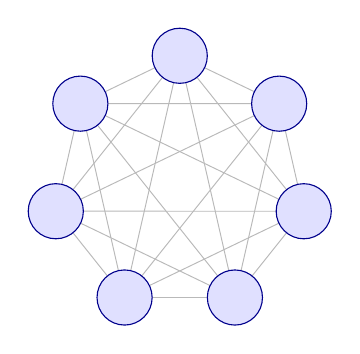
\begin{tikzpicture}[scale=0.85,
      cand/.style={circle,draw=blue!55!black,fill=blue!12,minimum size=7mm,inner sep=0pt},
      edge/.style={draw=gray!55,line width=0.35pt}]
    \foreach \i in {0,...,6} {
      \coordinate (P\i) at ({90-\i*51.43}:1.9);
    }
    \foreach \i in {0,...,6} {
      \foreach \j in {0,...,6} {
        \ifnum\i<\j
          \draw[edge] (P\i) -- (P\j);
        \fi
      }
    }
    \foreach \i in {0,...,6} {
      \node[cand] at (P\i) {};
    }
  \end{tikzpicture}
  \caption{Baseline: full self-attention. Every candidate connects to every
  other --- $\binom{N}{2}$ edges, $\Theta(N^2)$.}
\end{subfigure}
\hfill
\begin{subfigure}[t]{0.46\textwidth}
  \centering
  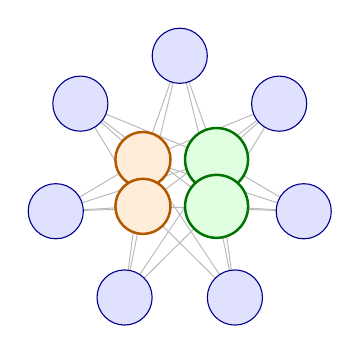
\begin{tikzpicture}[scale=0.85,
      cand/.style={circle,draw=blue!55!black,fill=blue!12,minimum size=7mm,inner sep=0pt},
      anchornode/.style={circle,draw=orange!70!black,fill=orange!15,minimum size=7mm,inner sep=0pt,line width=0.9pt},
      ctxnode/.style={circle,draw=green!45!black,fill=green!12,minimum size=8mm,inner sep=0pt,line width=0.9pt},
      edge/.style={draw=gray!55,line width=0.35pt}]
    \foreach \i in {0,...,6} {
      \coordinate (P\i) at ({90-\i*51.43}:1.9);
    }
    \coordinate (A1) at (-0.55,0.35);
    \coordinate (A2) at (-0.55,-0.35);
    \coordinate (M1) at (0.55,0.35);
    \coordinate (M2) at (0.55,-0.35);
    \foreach \i in {0,...,6} {
      \draw[edge] (P\i) -- (A1);
      \draw[edge] (P\i) -- (A2);
      \draw[edge] (P\i) -- (M1);
      \draw[edge] (P\i) -- (M2);
    }
    \foreach \i in {0,...,6} {
      \node[cand] at (P\i) {};
    }
    \node[anchornode] at (A1) {};
    \node[anchornode] at (A2) {};
    \node[ctxnode] at (M1) {};
    \node[ctxnode] at (M2) {};
  \end{tikzpicture}
  \caption{Proposed: anchor-token cross-attention. Candidates (blue) connect
  only to $K{=}2$ anchors (orange) and macro/portfolio tokens (green) ---
  $N(K{+}2)$ edges, $\Theta(N)$ for fixed $K$.}
\end{subfigure}
\caption{Attention connectivity, illustrated at a small $N$ for legibility.}
\label{fig:graphs}
\end{figure}

\subsection{Pipeline}

Figure~\ref{fig:pipeline} shows the full proposed forward pass. The
per-candidate GRU encoder, and the actor/critic heads, are unchanged from
the baseline; only the aggregation stage between them changes.

\begin{figure}[h!]
\centering
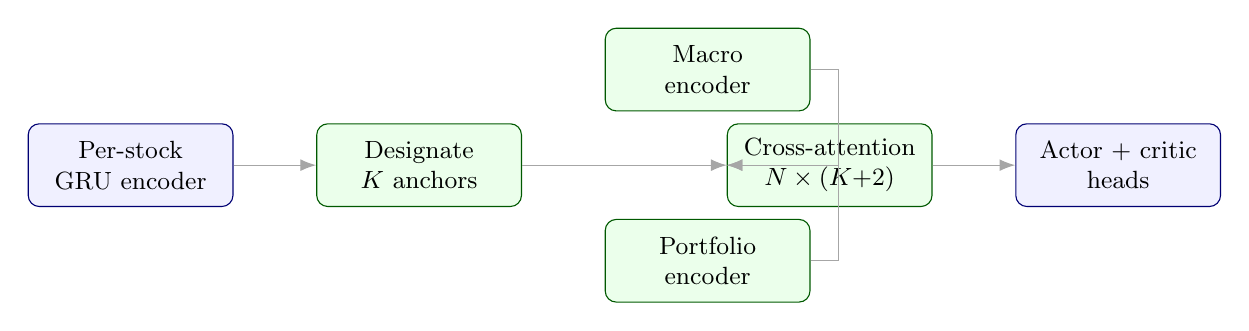
\begin{tikzpicture}[
    box/.style={draw, rounded corners, minimum width=2.6cm, minimum height=1.05cm,
                align=center, font=\small, inner sep=3pt},
    unchanged/.style={box, fill=blue!6, draw=blue!45!black},
    changed/.style={box, fill=green!8, draw=green!35!black},
    arr/.style={-{Latex[length=2mm]}, draw=gray!70}
  ]
  \node[unchanged] (gru) {Per-stock\\GRU encoder};
  \node[changed, right=1.05cm of gru] (anchor) {Designate\\$K$ anchors};
  \node[changed, above right=0.15cm and 1.05cm of anchor] (macro) {Macro\\encoder};
  \node[changed, below right=0.15cm and 1.05cm of anchor] (port) {Portfolio\\encoder};
  \node[changed, right=2.6cm of anchor] (attn) {Cross-attention\\$N\times(K{+}2)$};
  \node[unchanged, right=1.05cm of attn] (heads) {Actor $+$ critic\\heads};

  \draw[arr] (gru) -- (anchor);
  \draw[arr] (anchor.east) -- ++(0.35,0) |- (attn.west);
  \draw[arr] (macro.east) -- ++(0.35,0) |- (attn.west);
  \draw[arr] (port.east)  -- ++(0.35,0) |- (attn.west);
  \draw[arr] (attn) -- (heads);
\end{tikzpicture}
\caption{Proposed policy pipeline. Blue: unchanged from the baseline. Green:
new or restructured relative to Section~\ref{sec:baseline}.}
\label{fig:pipeline}
\end{figure}

% ─────────────────────────────────────────────────────────────────────────
\section{The Redesign Is Necessary but Not Sufficient}
\label{sec:linear-bottleneck}

Substituting Eq.~\eqref{eq:onk} for Eq.~\eqref{eq:on2} inside the fitted
model of Eq.~\eqref{eq:fit} --- reusing $c_0,c_1,c_2$ unchanged, since the
GRU/fusion/head costs they capture do not depend on the attention pattern,
and reusing $c_3$ as the measured per-key-value-pair cost of attention
itself --- gives a projected memory function for the proposed design:
\begin{equation}
  \widehat{\mathrm{mem}}_{\text{proposed}}(N,K,B) \;=\; c_0 + c_1 B + c_2(NB) + c_3\big(N(K+2)B\big).
  \label{eq:fit-proposed}
\end{equation}
As a consistency check, setting $K = N-2$ (a degenerate anchor set equal to
the whole candidate universe) recovers Eq.~\eqref{eq:fit} exactly, as it
must: $\widehat{\mathrm{mem}}_{\text{proposed}}(N,N{-}2,B) =
\widehat{\mathrm{mem}}(N,B)$.

Table~\ref{tab:projection} evaluates both models at $N{=}1500$, $K{=}8$.
The proposed design does reduce memory --- by roughly 16\,\% at $B{=}32$ ---
but \emph{both} figures exceed this GPU's usable ceiling. The reason is
visible directly in Eq.~\eqref{eq:fit-proposed}: at $N{=}1500$, the linear
term $c_2(NB)$ already dominates the total almost completely
($c_2 \cdot 1500 \cdot 32 \approx 24.4$\,GB, versus a quadratic-term
contribution, at $K{=}8$, of only $c_3\cdot1500\cdot10\cdot32\approx
0.031$\,GB). Eq.~\eqref{eq:onk}'s asymptotic improvement is real, but at
$N{=}1500$ it has already stopped being the binding constraint.

\begin{table}[h!]
\centering
\caption{Baseline vs.\ proposed, projected at $N{=}1500,K{=}8$.}
\label{tab:projection}
\begin{tabular}{@{}lrr@{}}
\toprule
 & Baseline (GB) & Proposed, $K{=}8$ (GB) \\
\midrule
$B=4$   & 3.63  & 3.06 \\
$B=8$   & 7.26  & 6.12 \\
$B=32$  & 29.04 & 24.46 \\
$B=256$ & 232.3 & 195.7 \\
\bottomrule
\end{tabular}
\end{table}

Solving Eq.~\eqref{eq:fit-proposed} for the largest batch size under a
memory budget $M$,
\begin{equation}
  B_{\max}(N,K,M) \;=\; \frac{M - c_0}{c_1 + c_2 N + c_3 N(K+2)},
  \label{eq:bmax}
\end{equation}
gives, at $N{=}1500,K{=}8$: $B_{\max}\approx11.4$ under the verified-safe
budget ($M{=}8.657$\,GB) and $B_{\max}\approx20.4$ under the raw usable
ceiling ($M{=}15.57$\,GB, subject to the Section~\ref{sec:caveat} caveat).
Neither approaches the batch sizes (128--256) that fit easily at $N{=}60$
today. Reaching them at $N{=}1500$ requires a second lever independent of
the attention redesign --- most plausibly a smaller per-candidate embedding
width, mixed-precision training, or gradient checkpointing through the GRU
--- which we leave as future work (Section~\ref{sec:discussion}).

% ─────────────────────────────────────────────────────────────────────────
\section{Training}
\label{sec:training}

The policy is trained with Proximal Policy Optimization
\citep{schulman2017ppo} using Generalized Advantage Estimation
\citep{schulman2016gae}; the loop is unaffected by the architecture change
proposed here beyond the forward-pass cost analyzed above.
Algorithm~\ref{alg:ppo} summarizes the current implementation
(\code{ppo.jl}, \code{train.jl}).

\begin{algorithm}[h!]
\caption{TradingGame training iteration}
\label{alg:ppo}
\begin{algorithmic}[1]
\State Roll out one full episode with the current policy, sampling
       $a^{\text{type}}_{i,t}\sim\mathrm{Categorical}(\mathrm{softmax}(\ell_{i,t}))$
       per candidate; record $(s_t,a_t,\log\pi_{\text{old}}(a_t|s_t),r_t,V(s_t))_{t=1}^{T}$
\State Compute advantages via GAE: $\delta_t = r_t + \gamma V(s_{t+1}) - V(s_t)$,
       $\hat{A}_t = \sum_{k\ge0}(\gamma\lambda)^k\delta_{t+k}$; normalize $\hat{A}_t$
\For{$K_{\text{epochs}}$ passes over shuffled minibatches}
  \State $\rho_t(\theta) \leftarrow \exp\big(\log\pi_\theta(a_t|s_t) - \log\pi_{\text{old}}(a_t|s_t)\big)$
  \State $\mathcal{L}^{\text{CLIP}} \leftarrow \mathbb{E}_t\big[\min(\rho_t\hat{A}_t,\;
         \mathrm{clip}(\rho_t,1{-}\epsilon,1{+}\epsilon)\hat{A}_t)\big]$
  \State $\mathcal{L} \leftarrow -\mathcal{L}^{\text{CLIP}} + c_v\,\mathbb{E}_t[(V_\theta(s_t)-\hat{R}_t)^2] - c_e\,\mathbb{E}_t[\mathcal{H}(\pi_\theta(\cdot|s_t))]$
  \State Update $\theta$ with Adam \citep{kingma2015adam}
\EndFor
\State Checkpoint if the (held-out, greedy) episode return improved
\end{algorithmic}
\end{algorithm}

The continuous buy-weight $w_{i,t}$ (Eq.~\eqref{eq:action-space}) is used
deterministically --- $w_{i,t}=\sigma(\text{logit})$, renormalized by the
masking layer --- rather than sampled from a second distribution; PPO's
log-probability ratio $\rho_t$ is computed over the categorical
$a^{\text{type}}$ choice only. This keeps the stochastic side of a hybrid
discrete/continuous action space tractable for a hand-rolled
implementation, at the cost of not learning position-sizing stochastically.
None of this changes under the proposed architecture, which affects only
how $s_t$ is encoded into $\ell_{i,t}$ and $V(s_t)$.

% ─────────────────────────────────────────────────────────────────────────
\section{Discussion and Open Questions}
\label{sec:discussion}

\begin{itemize}
  \item \textbf{Anchor selection.} Candidates include index constituents
    (e.g.\ Nifty~50), the top-$K$ candidates by market capitalization, or
    one representative per major sector. Any choice must be a subset of the
    episode's own candidate universe, so no extra encoding pass is needed.
  \item \textbf{Anchor stability.} Fixing $\mathcal{A}$ per episode keeps
    $K$ genuinely constant for Eq.~\eqref{eq:onk}'s accounting; re-selecting
    anchors more frequently (e.g.\ today's top movers) could be more
    informative but reopens a small $O(N)$ selection cost per step and makes
    the attended set non-stationary within an episode.
  \item \textbf{The linear bottleneck (Section~\ref{sec:linear-bottleneck})}
    is, on the evidence here, the harder remaining problem: it is intrinsic
    to encoding $N$ independent price histories, not to any particular
    cross-candidate mixing strategy.
  \item \textbf{GPU wiring.} \code{ppo.jl}/\code{train.jl} currently run
    entirely on CPU (a deliberate scoping decision for the initial PPO
    implementation); every measurement in this note characterizes the
    network in isolation, not the full rollout-and-update loop.
  \item \textbf{\code{assemble\_observation} is a separate, CPU-bound cost}
    --- a per-candidate Julia loop run once per environment step --- outside
    the scope of the GPU analysis here and worth profiling independently as
    $N$ grows.
\end{itemize}

% ─────────────────────────────────────────────────────────────────────────
\section{Conclusion}

Full self-attention across the candidate universe, as implemented today, is
quadratic in $N$ and --- measured directly, not merely argued asymptotically
--- exhausts a 16.7\,GB GPU at $N{=}1500$ between batch sizes 8 and 16.
Anchor-token cross-attention, restricted to a small fixed context set of
real anchor stocks plus separate macro and portfolio tokens, is linear in
$N$ and recovers exactly the selectivity a pooled-summary alternative would
have discarded. It reduces memory meaningfully (Table~\ref{tab:projection})
but does not, by itself, make $N{=}1500$ training cheap: a linear
per-candidate encoding cost, fit from the same measurements
(Eq.~\eqref{eq:fit}), remains and now dominates. Both findings --- the
quadratic bottleneck and its linear successor --- come from the same
thirteen-point empirical characterization and the same closed-form model,
which is the artifact we consider most durable here: not a specific
proposed architecture, but a validated method for answering "does this fit
on this GPU" without guessing.

\bibliographystyle{plainnat}
\bibliography{tradinggame_scaling}

\end{document}
